\ifx\allfiles\undefined
\documentclass[12pt, a4paper, oneside, UTF8]{ctexbook}
\def\path{../config}
\usepackage{amsmath}
\usepackage{amsthm}
\usepackage{array}
\usepackage{amssymb}
\usepackage{graphicx}
\usepackage{mathrsfs}
\usepackage{enumitem}
\usepackage{geometry}
\usepackage[colorlinks, linkcolor=black]{hyperref}
\usepackage{stackengine}
\usepackage{yhmath}
\usepackage{extarrows}
% \usepackage{unicode-math}
\usepackage{esint}
\usepackage{multirow}
\usepackage{fancyhdr}
\usepackage[dvipsnames, svgnames]{xcolor}
\usepackage{listings}
\usepackage{float} % Required for the H float option
\definecolor{mygreen}{rgb}{0,0.6,0}
\definecolor{mygray}{rgb}{0.5,0.5,0.5}
\definecolor{mymauve}{rgb}{0.58,0,0.82}
\definecolor{NavyBlue}{RGB}{0,0,128}
\definecolor{Rhodamine}{RGB}{255,0,255}
\definecolor{PineGreen}{RGB}{0,128,0}

\graphicspath{ {figures/},{../figures/}, {config/}, {../config/} }

\linespread{1.6}

\geometry{
    top=25.4mm, 
    bottom=25.4mm, 
    left=20mm, 
    right=20mm, 
    headheight=2.17cm, 
    headsep=4mm, 
    footskip=12mm
}

\setenumerate[1]{itemsep=5pt,partopsep=0pt,parsep=\parskip,topsep=5pt}
\setitemize[1]{itemsep=5pt,partopsep=0pt,parsep=\parskip,topsep=5pt}
\setdescription{itemsep=5pt,partopsep=0pt,parsep=\parskip,topsep=5pt}

\lstset{
    language=Mathematica,
    basicstyle=\tt,
    breaklines=true,
    keywordstyle=\bfseries\color{NavyBlue}, 
    emphstyle=\bfseries\color{Rhodamine},
    commentstyle=\itshape\color{black!50!white}, 
    stringstyle=\bfseries\color{PineGreen!90!black},
    columns=flexible,
    numbers=left,
    numberstyle=\footnotesize,
    frame=tb,
    breakatwhitespace=false,
} 

\lstset{
    language=TeX, % 设置语言为 TeX
    basicstyle=\ttfamily, % 使用等宽字体
    breaklines=true, % 自动换行
    keywordstyle=\bfseries\color{NavyBlue}, % 关键字样式
    emphstyle=\bfseries\color{Rhodamine}, % 强调样式
    commentstyle=\itshape\color{black!50!white}, % 注释样式
    stringstyle=\bfseries\color{PineGreen!90!black}, % 字符串样式
    columns=flexible, % 列的灵活性
    numbers=left, % 行号在左侧
    numberstyle=\footnotesize, % 行号字体大小
    frame=tb, % 顶部和底部边框
    breakatwhitespace=false % 不在空白处断行
}

% \begin{lstlisting}[language=TeX] ... \end{lstlisting}

% 定理环境设置
\usepackage[strict]{changepage} 
\usepackage{framed}

\definecolor{greenshade}{rgb}{0.90,1,0.92}
\definecolor{redshade}{rgb}{1.00,0.88,0.88}
\definecolor{brownshade}{rgb}{0.99,0.95,0.9}
\definecolor{lilacshade}{rgb}{0.95,0.93,0.98}
\definecolor{orangeshade}{rgb}{1.00,0.88,0.82}
\definecolor{lightblueshade}{rgb}{0.8,0.92,1}
\definecolor{purple}{rgb}{0.81,0.85,1}

\theoremstyle{definition}
\newtheorem{myDefn}{\indent Definition}[section]
\newtheorem{myLemma}{\indent Lemma}[section]
\newtheorem{myThm}[myLemma]{\indent Theorem}
\newtheorem{myCorollary}[myLemma]{\indent Corollary}
\newtheorem{myCriterion}[myLemma]{\indent Criterion}
\newtheorem*{myRemark}{\indent Remark}
\newtheorem{myProposition}{\indent Proposition}[section]

\newenvironment{formal}[2][]{%
	\def\FrameCommand{%
		\hspace{1pt}%
		{\color{#1}\vrule width 2pt}%
		{\color{#2}\vrule width 4pt}%
		\colorbox{#2}%
	}%
	\MakeFramed{\advance\hsize-\width\FrameRestore}%
	\noindent\hspace{-4.55pt}%
	\begin{adjustwidth}{}{7pt}\vspace{2pt}\vspace{2pt}}{%
		\vspace{2pt}\end{adjustwidth}\endMakeFramed%
}

\newenvironment{definition}{\vspace{-\baselineskip * 2 / 3}%
	\begin{formal}[Green]{greenshade}\vspace{-\baselineskip * 4 / 5}\begin{myDefn}}
	{\end{myDefn}\end{formal}\vspace{-\baselineskip * 2 / 3}}

\newenvironment{theorem}{\vspace{-\baselineskip * 2 / 3}%
	\begin{formal}[LightSkyBlue]{lightblueshade}\vspace{-\baselineskip * 4 / 5}\begin{myThm}}%
	{\end{myThm}\end{formal}\vspace{-\baselineskip * 2 / 3}}

\newenvironment{lemma}{\vspace{-\baselineskip * 2 / 3}%
	\begin{formal}[Plum]{lilacshade}\vspace{-\baselineskip * 4 / 5}\begin{myLemma}}%
	{\end{myLemma}\end{formal}\vspace{-\baselineskip * 2 / 3}}

\newenvironment{corollary}{\vspace{-\baselineskip * 2 / 3}%
	\begin{formal}[BurlyWood]{brownshade}\vspace{-\baselineskip * 4 / 5}\begin{myCorollary}}%
	{\end{myCorollary}\end{formal}\vspace{-\baselineskip * 2 / 3}}

\newenvironment{criterion}{\vspace{-\baselineskip * 2 / 3}%
	\begin{formal}[DarkOrange]{orangeshade}\vspace{-\baselineskip * 4 / 5}\begin{myCriterion}}%
	{\end{myCriterion}\end{formal}\vspace{-\baselineskip * 2 / 3}}
	

\newenvironment{remark}{\vspace{-\baselineskip * 2 / 3}%
	\begin{formal}[LightCoral]{redshade}\vspace{-\baselineskip * 4 / 5}\begin{myRemark}}%
	{\end{myRemark}\end{formal}\vspace{-\baselineskip * 2 / 3}}

\newenvironment{proposition}{\vspace{-\baselineskip * 2 / 3}%
	\begin{formal}[RoyalPurple]{purple}\vspace{-\baselineskip * 4 / 5}\begin{myProposition}}%
	{\end{myProposition}\end{formal}\vspace{-\baselineskip * 2 / 3}}


\newtheorem{example}{\indent \color{SeaGreen}{Example}}[section]
\renewcommand{\proofname}{\indent\textbf{\textcolor{TealBlue}{Proof}}}
\newenvironment{solution}{\begin{proof}[\indent\textbf{\textcolor{TealBlue}{Solution}}]}{\end{proof}}

% 自定义命令的文件

\def\d{\mathrm{d}}
\def\R{\mathbb{R}}
%\newcommand{\bs}[1]{\boldsymbol{#1}}
%\newcommand{\ora}[1]{\overrightarrow{#1}}
\newcommand{\myspace}[1]{\par\vspace{#1\baselineskip}}
\newcommand{\xrowht}[2][0]{\addstackgap[.5\dimexpr#2\relax]{\vphantom{#1}}}
\newenvironment{mycases}[1][1]{\linespread{#1} \selectfont \begin{cases}}{\end{cases}}
\newenvironment{myvmatrix}[1][1]{\linespread{#1} \selectfont \begin{vmatrix}}{\end{vmatrix}}
\newcommand{\tabincell}[2]{\begin{tabular}{@{}#1@{}}#2\end{tabular}}
\newcommand{\pll}{\kern 0.56em/\kern -0.8em /\kern 0.56em}
\newcommand{\dive}[1][F]{\mathrm{div}\;\boldsymbol{#1}}
\newcommand{\rotn}[1][A]{\mathrm{rot}\;\boldsymbol{#1}}

% 修改参数改变封面样式,0 默认原始封面、内置其他1、2、3种封面样式
\def\myIndex{0}


\ifnum\myIndex>0
    \input{\path/cover_package_\myIndex}
\fi

\def\myTitle{标题:一份LaTeX笔记模板}
\def\myAuthor{作者名称}
\def\myDateCover{封面日期: \today}
\def\myDateForeword{前言页显示日期: \today}
\def\myForeword{前言标题}
\def\myForewordText{
    
    这是一个基于\LaTeX{}的模板,用于撰写学习笔记。

    模板旨在提供一个简单、易用的框架,以便你能够专注于内容,而不是排版细节,如不是专业者,不建议使用者在模板细节上花费太多时间,而是直接使用模板进行笔记撰写。遇到问题,再进行调整解决。
}
\def\mySubheading{副标题}


\begin{document}
% \input{\path/cover_text_\myIndex.tex}

\newpage
\thispagestyle{empty}
\begin{center}
    \Huge\textbf{\myForeword}
\end{center}
\myForewordText
\begin{flushright}
    \begin{tabular}{c}
        \myDateForeword
    \end{tabular}
\end{flushright}

\newpage
\pagestyle{plain}
\setcounter{page}{1}
\pagenumbering{Roman}
\tableofcontents

\newpage
\pagenumbering{arabic}
\setcounter{chapter}{-1}
\setcounter{page}{1}

\pagestyle{fancy}
\fancyfoot[C]{\thepage}
\renewcommand{\headrulewidth}{0.4pt}
\renewcommand{\footrulewidth}{0pt}








\else
\fi

\chapter{混凝土}

\section{普通混凝土的基本组成材料}

\begin{definition}
    混凝土的狭义定义是:水泥、粗骨料、细骨料和水按一定比例混合而成的材料。

    水泥和水组成水泥浆,填充骨料之间的空隙。在混凝土硬化前,水泥浆起润滑作用,赋于混凝土拌合物流动性,便于施工;在混凝土硬
    化后起胶结作用,把砂、石骨料胶结成为整体,使混凝土产生强度,成为坚硬的人造石材。砂、石是骨料,对混凝土起骨架作用,
\end{definition}

\begin{remark}
    氯离子对钢筋有腐蚀作用,不宜用海砂。
\end{remark}

\begin{definition}
    细度模数$M_x = \frac{(A_2 + A_3 + A_4 + A_5 + A_6) - 5A_1}{100 - A_1}$

    将500g干砂试样由粗到细依次过筛,然后称得剩留在各个筛上的砂重量(m),并计算出各筛上的分汁筛余百分率(各筛上的筛余量占砂样重的百分率),分别以a表示。再算出各筛的累计筛余百分率(各个筛与比该筛粗的所有筛之分计筛余百分率之和),分别以A表示。
$$
a_i=\frac{m_i}{500}\times100 \%,
\textnormal{显然}A_j=\sum_{i=1}^{j}a_i
$$

细度模数是衡量砂粗细程度的指标。细度模数愈大,表示砂愈粗。({\color{red}粗砂3.7- 3.1,中砂3.0-2.3,细砂2.2-1.6})
\end{definition}

\begin{remark}
    砂骨料的含水状态:

   (1)干燥状态:含水率等于或接近于零

   (2)气干状态:含水率与大气湿度相平衡

   (3)饱和面干状态:骨料表面干燥而内部孔隙含水达到饱和

   (4)湿润状态:不仅内部孔隙充满水,表面附有一层表面水
\end{remark}

\textbf{粗骨料:}

\begin{enumerate}
    \item 有害物质:卵石和碎石中不应混有草根、树叶、树枝、塑料、煤块和炉渣等杂物。
    \item 碱骨料反应:水泥中的碱性氧化物与骨料中的活性成分反应,生成碱-硅酸凝胶体,它会吸水肿胀产生膨胀。使用含碱量小于0.6%的水泥,或掺加能抑制碱—骨料反应的
    掺合料。
    \item 混凝土用粗骨料其颗粒形状以接近立方形或球形的为好,而针状和片状颗粒含量要少。否则会降低强度。
    \item 骨料表面特征:与碎石比较(碎石多棱角),卵石表面光滑,拌制混凝土时需用水泥浆量较少,拌合物和易性较好。但是强度没有碎石高。
\end{enumerate}

\section{混凝土的技术性质}

\begin{definition}
    影响混凝土流动性的因素:

    混凝土拌合物内的阻力主要来自两个方面,一为骨料间的摩阻力,一为水泥浆的粘聚力。

    \begin{enumerate}
        \item 水泥浆数量:在水灰比不变的情况下,如果水泥浆越多,则拌合物的流动性越大。但若水泥浆过多,使拌合物的粘聚性变差。老师提到了,水泥浆早期是起润滑作用,后期才是起胶结作用。{\color{red}这条我是感觉有点反常识的,毕竟配比是不变的,但是绝对数量是影响的}
        \item 水灰比:在水泥用量不变的情况下,水灰比越小,水泥浆就越稠厚,水泥浆的流动性就越差,混凝土的流动性也就越差。
        \item 水泥性质:例如采用矿渣水泥或
        火山灰水泥拌制的混凝土拌合物,其流动性比用普通水泥时为小,这是因为前者水泥的密度较小
        ,所以在相同水泥用量时,它们的绝对体积较大,且在相同稠度下需水量要大一些,因此混凝土
        就显得较稠。
        \item 砂率:砂起到填充大石头间隙的作用,{\color{red}所以砂率应当有一个最合适的值},过大过小都不好。
        \item 骨料性质:采用卵石和河砂拌制的混凝土拌合物,其流动性比用碎
        石和山砂拌制的好,这是因为前者骨料表面光滑,摩阻力小;用级配好的骨料拌制的混凝土拌合
        物和易性好,因为骨料级配好时其空隙少。
        \item 拌合物存放时间及环境温度的影响:随着时间的延长,流动性下降(温度过高,水分丧失)。
        \item 外加剂的影响:混凝土拌合物掺入减水剂或引气剂,流动性明显提高,引气剂还可有效地改善混凝土拌合物的粘聚性和保水性,二者还分别对硬化混凝土的强度与耐久性起着十分有利的作用。
    \end{enumerate}
\end{definition}

\textbf{混凝土拌合物的和易性(工作性)}

定义:是指混凝土拌合物能保持其组成成分均匀,不发生分层离析、泌水等现象,适于运输、浇筑、捣实成型等施工作业,并能获得质量均匀、密实的混凝土的性能。和易性为一个综合技术性能,它包括流动性、粘聚性和保水性三方面的涵义。
\begin{enumerate}
    \item 流动性:是指混凝土拌合物在自重或机械振捣力的作用下,能产生{\color{red}流动并均匀密实地充满模型的性能}。混凝土拌合物的流动性以坍落度或维勃稠度作为指标。坍落度适用于流动性较大的混凝土拌合物,维勃稠度适用于干硬的混凝土拌合物。
    \item 粘聚性:是指混凝土拌合物{\color{red}内部组分间的粘聚力},在运输和浇筑过程中不致发生离析分层现象,而使混凝土能保持整体均匀的性能。
    \item 保水性:是指混凝土拌合物{\color{red}保持内部水分}、在施工过程中不致产生严重的泌水现象的能力。
\end{enumerate}

\begin{theorem}
无论是水泥浆数量的影响,还是水泥浆稠度的影响,实际上都是水的影响。因此,影响混凝土拌合物和易性的决定性因素是其拌合用水量的多少。

实践证明,在配制混凝土时,当所用粗、细骨料的种类及比例一定时,为获得要求的流动性,所需拌合用水量基本是一定的,即使水泥用量有所变动时,也无甚影响。这一关系称为“恒定用水量法则”,它为混凝土配合比设计时确定拌合用水量带来很大方便。{\color{red}粗骨料的需要更少的水,这是因为粗骨料的总表面积比细骨料更小,只要更少的水来包裹}。
\end{theorem}

\textbf{改善流动性的措施:}

(1)尽可能选用较粗大的粗、细骨料;

(2)采用泥及泥块等杂质含量少,级配好的粗、细骨料;

(3)尽量降低砂率;

(4)在上述基础上,保持水灰比不变,适当增加水泥用量和用水量;如流动性太大,则保持砂率不变,适当增加砂、石用量;

(5)掺加减水剂。

\textbf{改善粘聚性和保水性的措施:}

(1)选用级配良好的粗、细骨料,并选用连续级配;

(2)适当限制粗骨料的最大粒径,避免选用过粗的细骨料;

(3)适当增大砂率或掺加粉煤灰等矿物外加剂;

(4)掺加减水剂和引气剂。

\begin{table}[H]
    \centering
    \begin{tabular}{|c|c|c|}
    \hline
    \textbf{外加剂类型} & \textbf{主要作用} & \textbf{作用机理} \\
    \hline
    减水剂 & 减少水分,增加强度,增强耐久性。 & 吸附分散作用、润滑作用\\
    \hline
    早强剂 & 调节凝结硬化速率 & 促进水泥的水化和硬化\\
    \hline
    引气剂 & 提高抗渗性,提高抗冻性 & 增加小气泡,降低摩擦\\
    \hline
    防冻剂 & 提高抗冻性能 & 添加早强、减水、防冻、引气成分\\
    \hline
    膨胀剂 & 抵抗收缩,防止开裂 & 使水泥浆体膨胀\\
    \hline
    掺和料 & 减少水泥用量、降低成本 & 减少活性成分比例\\
    \hline
    减缩剂 & 减少混凝土收缩 & 物理减缩\\
    \hline
    \end{tabular}
    \caption{外加剂的作用及机理}
\end{table}

\textbf{减水剂的原理:}

水泥加水后,由于水泥颗粒在水中的热运动,使水泥颗粒之间在分子力的作用下,形成了一些絮凝状结构。降低了水泥的流动性,不得不加大量的水以保持和易性。
减水剂的本质是表面活性剂,亲水部分指向水溶剂,憎水部分指向水泥,起到了水泥颗粒之间的润滑作用。
同时减水剂所带的电荷打开了水泥的絮凝结构,释放了原来被束缚的游离水。

水泥颗粒在此作用下充分分散,提高了水化面积,减少了拌合水量,提高了水泥强度。(常见的有木质素系减水剂等)

\subsection{影响混凝土强度的因素}

1) 水泥强度: 水泥强度的大小直接影响混凝土强度的高低。在配合比相同的条件下,所用的水泥强度等级越高,制成的混凝土强度也越高。

2) 水灰比: 高水灰比导致低强度,由于工程中加水后水分蒸发会产生孔隙,导致强度下降。

3)骨料的种类、质量和数量:骨料级配良好可以产生更高强度。同时碎石由于比卵石更加粗糙,粘结力更强,可以产生更大强度。

4)外加剂和掺合料:
混凝土中加入外加剂可按要求改变混凝土的强度及强度发展规律,如掺入减水剂可减少拌合用水量,提高混凝土强度;如掺入早强剂可提高混凝土早期强度,但对其后期强度发展无明显影响。超细的掺合料可配制高性能、超高强度的混凝土。

5)施工条件:
在施工过程中,必须将混凝土拌合物搅拌均匀,浇注后必须捣固密实,才能使混凝土有达到预期强度的可能。机械搅拌和捣实的力度比人力要强(因为搅拌更加均匀)

6)养护条件:
养护环境温度高,水泥水化速度加快,混凝土早期强度高;反之亦然。若温度在冰点以下,不但水泥水化停止,而且有可能因冰冻导致混凝土结构疏松,强度严重降低,尤其是早期混凝土应特别加强防冻措施。为加快水泥的水化速度,可采用湿热养护的方法,即蒸汽养护或蒸压养护。湿度通常指的是空气相对湿度。相对湿度低,混凝土中的水份挥发快,混凝土因缺水而停止水化,强度发展受阻。另一方面,混凝土在强度较低时失水过快,极易引起干缩,影响混凝土耐久性。一般在混凝土浇筑完毕后12h内应开始对混凝土加以覆盖或浇水。对硅酸盐水泥、普通水泥和矿渣水泥配制的混凝土浇水养护不得少于7天;使用粉煤灰水泥和火山灰水泥,或掺有缓凝剂、膨胀剂、或有防水抗渗要求的混凝土浇水养护不得少于14天。

\begin{figure}[H]
	\centering
	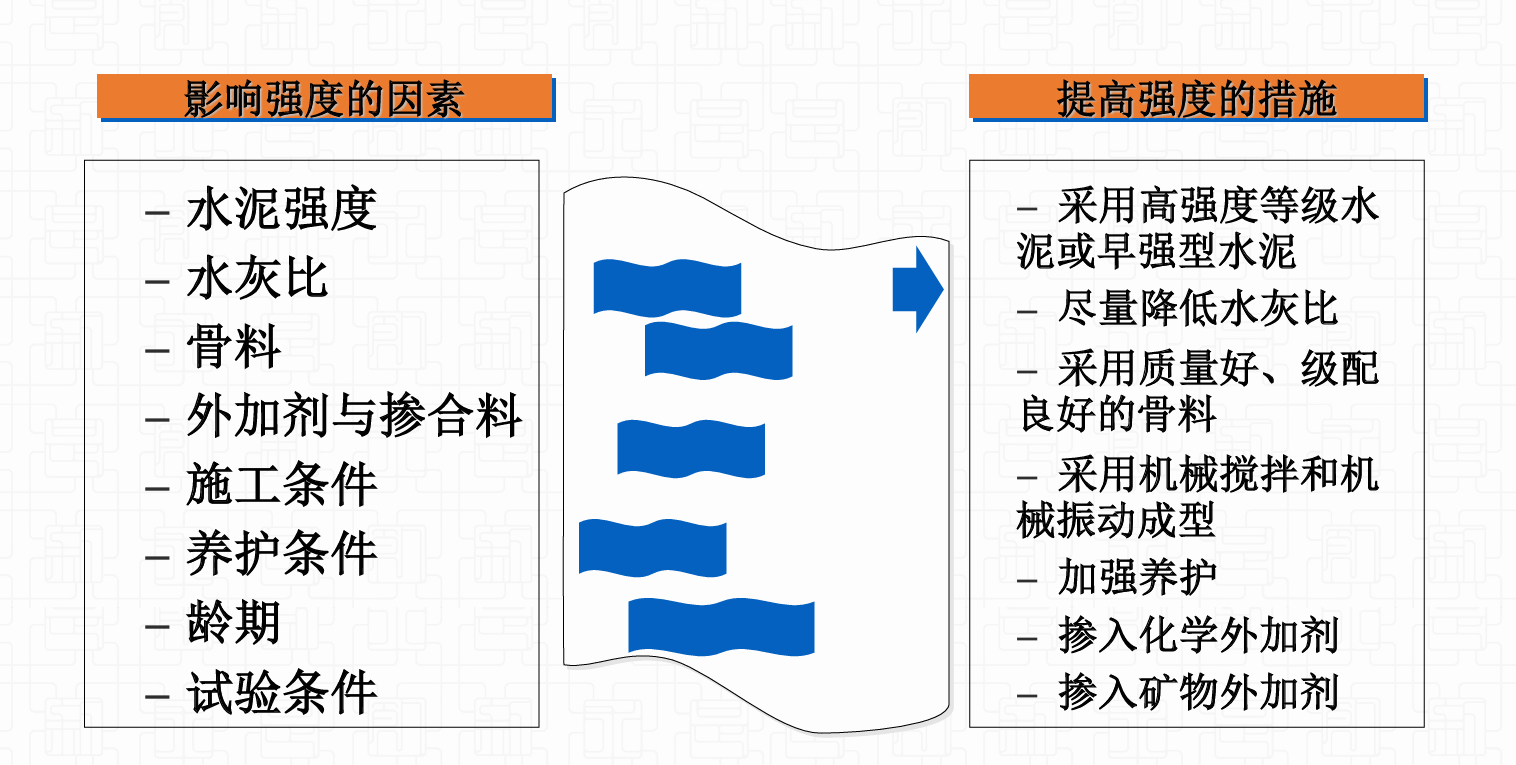
\includegraphics[width=0.7\linewidth]{../figure/qiangdu.png} % Ensure the file exists at this path
	\caption{混凝土强度影响因素}
	\label{fig:qiangdudengji}
\end{figure}

\textbf{计算强度经验公式:}
$$ f_{cu,28} = \alpha_{a} f_{ce} (B/W - \alpha_{b}) $$

式中 $f_{cu,28}$ —— 标准养护 28d 后的混凝土抗压强度,MPa;

$B/W$ —— 混凝土的胶水比(胶凝材料与水的质量之比);

$\alpha_{a}$、$\alpha_{b}$ —— 与粗骨料有关的回归系数,可通过历史资料统计得到,若无统计资料,可采用《普通混凝土配合比设计规程》(JGJ 55—2011)提供的经验值:采用碎石时 $\alpha_{a} = 0.53$,$\alpha_{b} = 0.20$;采用卵石时 $\alpha_{a} = 0.49$,$\alpha_{b} = 0.13$;

$f_{ce}$ —— 实测的经标准养护 28d 的胶凝材料胶砂抗压强度(MPa)。无实验条件时,可取 $f_{ce}= \gamma_{f} \gamma_{s} \gamma_{c} f_{ce,k}$
,其中 $f_{ce,k}$ 为水泥强度等级标准值;$\gamma_{c}$ 为与水泥强度等级值有关的强度富余系数。
$\gamma_{f}$ 和 $\gamma_{s}$ 分别为掺加粉煤灰和矿渣微粉作为混凝土掺合料时,对胶凝材料胶砂强度的影响系数。

\begin{remark}
    根据早期强度推算 28d 龄期强度公式:
$$
\frac{f_{cu}}{f_n} = \frac{\lg 28}{\lg n}
$$
式中 $n$ 为第 $n$ 天龄期
\end{remark}

\newpage

\subsection{混凝土耐久性的影响因素}

\begin{definition}
混凝土的耐久性

定义:混凝土在长期外界因素作用下,抵抗外部和内部不利影响的能力。

\begin{enumerate}
    \item 抗渗性:水的渗入可能导致水泥水化产物的溶解,可能导致软水腐蚀,也可能直接腐蚀钢筋,或者渗入水导致冻融作用侵蚀。
    \item 抗冻性:硬化混凝土在水饱和状态下,经受多次冻融循环而不破坏、同时也不严重降低强度的性能。
    \item 抗侵蚀性:混凝土抵抗各种酸、碱、盐液体或气体侵蚀的能力。
    \item 抗碳化性:氢氧化钙转变为碳酸钙的过程(实际上还有水化硅酸钙以及钙矾石也转变为碳酸钙)。好处是强度提高了,坏处是体积收缩导致裂缝,同时碱度下降,导致钢筋表面钝化膜消失,产生锈蚀。
    \item 碱骨料反应:混凝土内水泥中的碱性氧化物($Na_2O$、$K_2O$),与骨料中的活性SiO₂发生化学反应,生成碱——硅酸凝胶,其吸水后产生很大的体积膨胀,从而导致混凝土产生膨胀开裂而破坏的现象。
\end{enumerate}
\end{definition}

\textbf{提高混凝土耐久性的主要措施:}

混凝土材料

结构构造和裂缝宽度限制

施工要求

特殊防腐蚀措施

\section{混凝土质量控制}
用数理统计方法可求出几个特征统计量:强度平均值、强度标准差 (σ) 以及变异系数 ($C_v$)。强度标准差越大,说明强度的离散程度越大,混凝土质量愈不均匀。也可用变异系数来评定,该值越小,混凝土质量愈均匀。

\begin{remark}
    对于强度标准差,显然越小品控越好。对应的正态分布曲线越窄越高。

    $C_v = \frac{\sigma}{\bar{f_{CU}}}$
\end{remark}

对于强度保证率,有假定正态分布和假定使用样本近似的两种方法:

\begin{figure}[H]
	\centering
	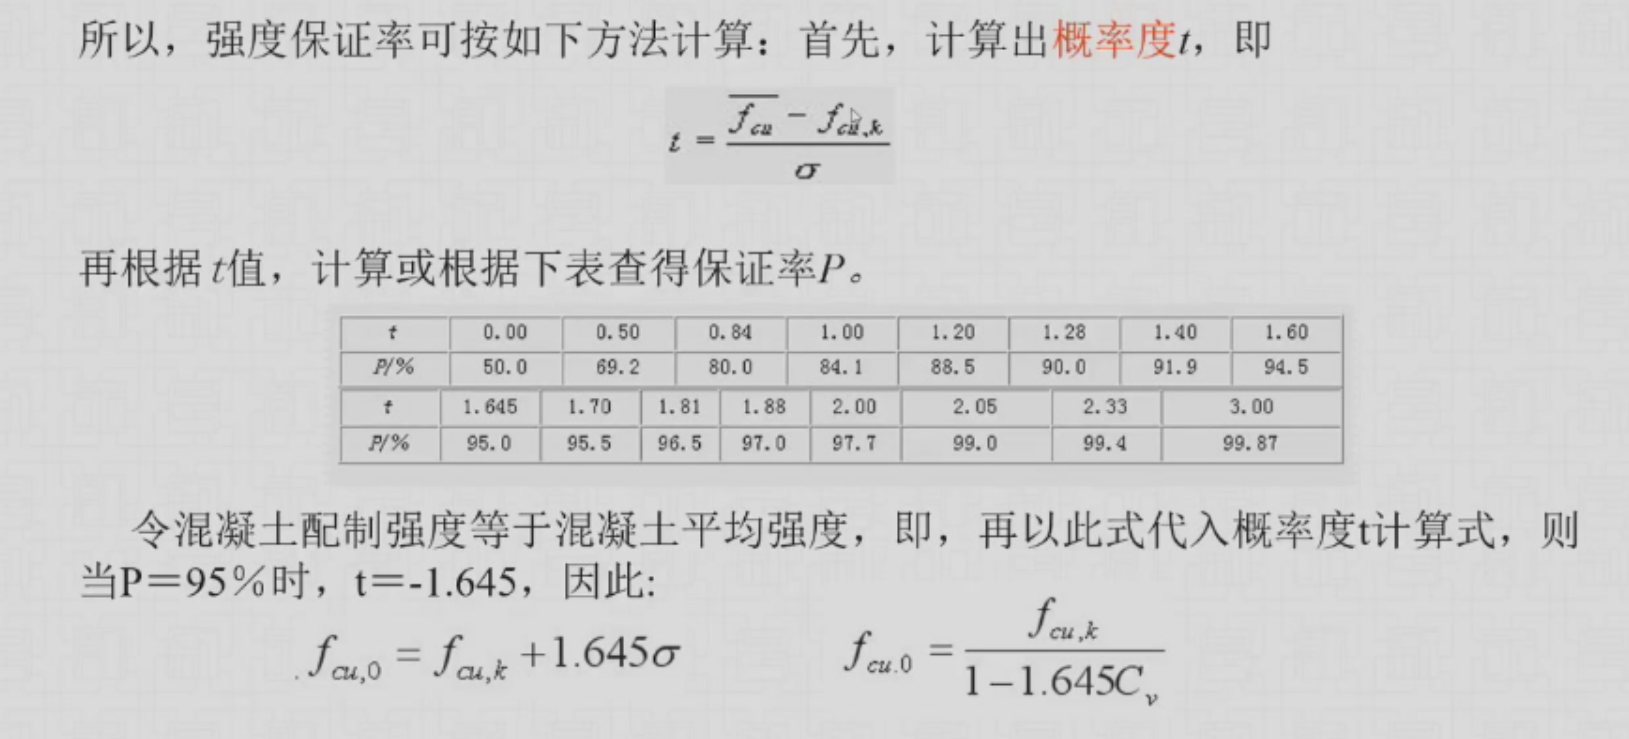
\includegraphics[width=0.9\linewidth]{../figure/tzhibiao.png} % Ensure the file exists at this path
	\caption{强度保证率计算方法其一}
	\label{fig:tzhibiao}
\end{figure}

比如说,工厂要求是10 MPa,你应当使用10MPa+ 1.645$\sigma$(这里$\sigma$是工厂生产的混凝土的标准差),以便确保有95\%的概率达到10MPa的强度。

\begin{figure}[H]
	\centering
	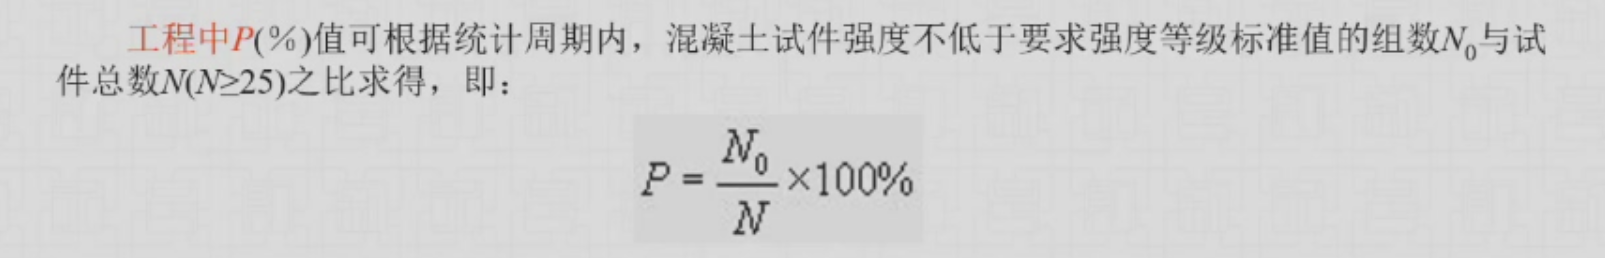
\includegraphics[width=0.9\linewidth]{../figure/SAA.png} % Ensure the file exists at this path
	\caption{强度保证率计算方法其二}
	\label{fig:SAA}
\end{figure}

\section{混凝土配比}
\begin{theorem}
\paragraph{基本要求}
包括:和易性、强度、耐久性、经济性(最后考虑)。
\paragraph{基本参数}
包括:水灰比、单位用水量和砂率。
\end{theorem}

顺序是先依据刚才的强度保证率,计算得到强度,根据强度反算水胶比,然后确定用水量,依据用水量和水胶比反算胶凝材料、矿物掺合料和水泥用量,确定砂石用量。

1. 确定混凝土配制强度
\[ f_{cu,0} = \begin{cases}f_{cu,k} + 1.645 \sigma & (f_{cu,k} < C60) \\  1.15 f_{cu,k} & (f_{cu,k} \geq C60)  \end{cases}\]

2. 确定水胶比
\[ \frac{W}{B} = \frac{\alpha_{a} f_{ce}}{f_{cu,0} + \alpha_{a} \alpha_{b} f_{ce}} \]
无实测值时,\( f_{b} = \gamma_{f} \gamma_{s} f_{ce}, f_{ce} = \gamma_{c} f_{ce,g} \)
同时应符合 \( \leq (W/B)_{\text{max}} \) 的要求

3. 确定混凝土拌和用水量 \( m_{w0} \)(查表得到;掺外加剂时计算得到,具体见后)

4. 计算胶凝材料、矿物掺合料和水泥用量
\[ m_{b0} = \frac{m_{w0}}{W/B} \]
同时应 \( \geq (m_{b0})_{\text{min}} \)

5. 确定合理砂率 \( \beta_{s} \)(查表得到或计算得到)
\[ m_{f0} = m_{b0} \beta_{f} \]
\[ m_{c0} = m_{b0} - m_{f0} \]

6. 计算砂石用量\\

\begin{remark}
    W/B的值不仅由强度确定,还由耐久性决定,两者取最小值。
\end{remark}

\newpage

\begin{tabular}{|c|p{10cm}|}
\hline
\textbf{符号} & \textbf{含义} \\ 
\hline
$f_b$ & 混凝土抗压强度设计值 \\ 
\hline
$\gamma_f$ & 抗压强度安全系数 \\ 
\hline
$\gamma_s$ & 结构安全系数 \\ 
\hline
$f_{ce}$ & 混凝土等效抗压强度 \\ 
\hline
$\gamma_c$ & 材料安全系数 \\ 
\hline
$f_{ce,g}$ & 标准混凝土抗压强度(实验室28天标准养护测得) \\ 
\hline
$f_{cu}$ & 混凝土极限抗压强度(“cu”=ultimate) \\ 
\hline
$f_{cu,0}$ & 混凝土极限抗压强度的初始值(考虑了强度保证率的情况) \\ 
\hline
$f_{cu,k}$ & 混凝土极限抗压强度的特征值(生产的混凝土的参数) \\ 
\hline
\end{tabular}

计算时候考虑两种方法:

体积法:
\[
\frac{m_{c0}}{\rho_c} + \frac{m_{f0}}{\rho_f} + \frac{m_{w0}}{\rho_w} + \frac{m_{s0}}{\rho_s} + \frac{m_{g0}}{\rho_g} + 0.01\alpha = 1 (\rho \text{单位用} Kg/m^3) \text{(无引气时} \alpha = 1)
\]
\[
\beta_s = \frac{m_{s0}}{m_{s0} + m_{g0}}
\]
重量法(假定表观密度法)
\[
m_{c0} + m_{f0} + m_{w0} + m_{s0} + m_{g0} = m_{cp}
\]
\[
\beta_s = \frac{m_{s0}}{m_{s0} + m_{g0}}
\]

\begin{tabular}{|c|p{10cm}|}
\hline
\textbf{符号} & \textbf{含义} \\ 
\hline
$m_{c0}$ & 水泥的质量(单位:kg) \\ 
\hline
$m_{f0}$ & 外加剂的质量(单位:kg) \\ 
\hline
$m_{w0}$ & 水的质量(单位:kg) \\ 
\hline
$m_{s0}$ & 细集料的质量(单位:kg) \\ 
\hline
$m_{g0}$ & 粗集料的质量(单位:kg) \\ 
\hline
$\rho_c$ & 水泥的密度(单位:kg/m\(^3\)) \\ 
\hline
$\rho_f$ & 外加剂的密度(单位:kg/m\(^3\)) \\ 
\hline
$\rho_w$ & 水的密度(单位:kg/m\(^3\)) \\ 
\hline
$\rho_s$ & 细集料的密度(单位:kg/m\(^3\)) \\ 
\hline
$\rho_g$ & 粗集料的密度(单位:kg/m\(^3\)) \\ 
\hline
$\alpha$ & 引气率(无引气时,$\alpha = 1$) \\ 
\hline
$\beta_s$ & 细集料与总集料的质量比 \\ 
\hline
$m_{cp}$ & 混凝土的总质量(单位:kg) \\ 
\hline
\end{tabular}

体积法是基于混凝土各组成材料的体积比例来设计混凝土配比。具体来说,通过已知材料的质量和密度,计算出每种材料的体积,然后调整各材料的体积比,确保混凝土最终的体积为1立方米。

\begin{equation}
\frac{m_{c0}}{\rho_c} + \frac{m_{f0}}{\rho_f} + \frac{m_{w0}}{\rho_w} + \frac{m_{s0}}{\rho_s} + \frac{m_{g0}}{\rho_g} + 0.01\alpha = 1
\end{equation}

这表示混凝土的总体积等于1立方米,考虑了不同组分的体积和相应的密度。每个材料的质量(如水泥、外加剂、水、细集料、粗集料)除以它们的密度得到体积,再加上引气量(由$\alpha$表示)来进行调整。$\alpha$是引气率,当没有使用引气时,$\alpha=1$。

重量法是根据各组分的质量来设计混凝土配比。该方法假定各材料的表观密度已经考虑了材料的干湿状态、孔隙度等影响,因此只需要根据各组成材料的质量来调整其比例,使得总质量满足设计要求。

\begin{equation}
m_{c0} + m_{f0} + m_{w0} + m_{s0} + m_{g0} = m_{cp}
\end{equation}

在重量法中,所有组分(如水泥、外加剂、水、细集料、粗集料)的质量之和等于混凝土的总质量 $m_{cp}$。与体积法不同,重量法直接通过质量来控制混凝土的组成,通常用于常规的混凝土设计中。

\begin{example}
    导致混凝土腐蚀的原因和反应有什么?

    按严重程度从高到低:

    \begin{enumerate}
    \item \textbf{碱-骨料反应 (Alkali-Aggregate Reaction, AAR)}\\
    混凝土中的碱性物质(如氢氧化钠、氢氧化钾)与骨料中的活性矿物反应,生成吸水膨胀的凝胶。这种凝胶在吸水后体积膨胀,导致混凝土内部产生膨胀应力,产生裂缝和剥落,严重破坏混凝土的结构完整性,是混凝土最严重的一种内部侵蚀。

    \item \textbf{硫酸盐侵蚀}\\
    硫酸盐离子渗入混凝土,与水泥中的氢氧化钙和三钙铝酸盐反应,生成膨胀性的硫酸钙类矿物(如石膏、钙矾石)。这些矿物体积膨胀,导致混凝土开裂和剥落,严重破坏混凝土结构。硫酸盐侵蚀在含硫酸盐环境中极具危害性,破坏程度与碱骨料反应相近。

    \item \textbf{碳化 (Carbonation)}\\
    大气中的二氧化碳与混凝土中的氢氧化钙反应生成碳酸钙:
    \[
    \mathrm{Ca(OH)_2 + CO_2 \rightarrow CaCO_3 + H_2O}
    \]
    该反应使混凝土孔隙被碳酸钙填充,增强了混凝土强度,但同时降低了混凝土的碱性(pH值下降),破坏了保护钢筋的氧化膜,易导致钢筋锈蚀,影响结构耐久性。
\end{enumerate}
\end{example}

\begin{example}
    为什么不能往混凝土加水,这和洒水养护矛盾吗?

往拌合好的混凝土中直接加水,会破坏它原先设计好的水胶比,进而带来一系列不利影响,而洒水养护则是混凝土达到初凝后,为了继续保证水化反应而在表面补充水分,防止因为水分的蒸发而导致反应不充分,导致强度不达标。两者并不矛盾。
\end{example}


\ifx\allfiles\undefined
\end{document}
\fi